\documentclass[10pt,journal,compsoc,onecolumn]{IEEEtran}
\usepackage[utf8]{inputenc}
\usepackage{amsmath,amsfonts,amssymb}
\usepackage{amsthm}
\usepackage{graphicx}
\usepackage{cite}
\usepackage{textcomp}
\usepackage{tikz}
\usetikzlibrary{arrows,positioning,shapes.geometric}
\usepackage{booktabs}
\usepackage{url}

\newtheorem{theorem}{Theorem}
\newtheorem{lemma}[theorem]{Lemma}
\newtheorem{definition}[theorem]{Definition}
\newtheorem{corollary}[theorem]{Corollary}

\begin{document}

\title{Depth-First Search on Binary Trees: Recursive and Iterative Traversal Algorithms, Call Stack Mechanics, and Practical Applications}

\IEEEtitleabstractindextext{%
\begin{abstract}
Depth-First Search (DFS) is a fundamental graph and tree traversal paradigm that explores as far as possible along each branch before backtracking. When applied to binary trees, DFS manifests in three canonical orderings: Pre-order (Root-Left-Right), In-order (Left-Root-Right), and Post-order (Left-Right-Root). This paper presents a rigorous formal analysis of all three DFS strategies on binary trees. We provide complete recursive Java implementations and trace their execution through detailed dry-run analyses, illustrating the call stack frame-by-frame. We then develop iterative (non-recursive) versions of each traversal using explicit stack data structures, proving their equivalence to the recursive formulations. For In-order traversal, we present Morris Traversal --- a $O(1)$ auxiliary space algorithm that uses temporary threaded links to eliminate both recursion and explicit stacks. We analyze the time complexity ($O(N)$ for all variants) and space complexity ($O(H)$ for recursive/stack-based, $O(1)$ for Morris). We further formalize DFS-based solutions to classic tree problems including height computation, diameter calculation, path sum detection, and tree construction from traversal pairs. All algorithms are implemented in Java with formal correctness proofs and illustrative TikZ diagrams.
\end{abstract}

\begin{IEEEkeywords}
linked list, deep copy, random pointer, hash map, node interleaving, Java, algorithm analysis, computational complexity
\end{IEEEkeywords}
}

\maketitle
\IEEEdisplaynontitleabstractindextext
\IEEEpeerreviewmaketitle

\section{Introduction}
Depth-First Search (DFS) is one of the two fundamental traversal paradigms for trees and graphs, the other being Breadth-First Search (BFS). While BFS explores all neighbors at the current depth before moving deeper (using a queue), DFS dives as deep as possible into a branch before backtracking (using a stack, either implicit via recursion or explicit).

In the context of binary trees, DFS is the natural traversal approach because the recursive structure of a binary tree --- where each node is the root of two sub-trees --- directly maps to recursive DFS calls. The three canonical DFS orderings differ only in \emph{when} the root node is processed relative to its subtrees:

\begin{itemize}
    \item \textbf{Pre-order (NLR):} Process the root \emph{before} its subtrees.
    \item \textbf{In-order (LNR):} Process the root \emph{between} its subtrees.
    \item \textbf{Post-order (LRN):} Process the root \emph{after} its subtrees.
\end{itemize}

Understanding DFS is critical for solving a wide class of algorithmic problems on trees: computing heights, diameters, path sums, lowest common ancestors, serialization, and tree construction from traversal sequences.

This paper provides a formal treatment across six sections. Section~\ref{sec:node} defines the binary tree node structure. Section~\ref{sec:recursive} presents all three recursive DFS traversals with dry-run traces. Section~\ref{sec:callstack} dissects the call stack mechanics. Section~\ref{sec:iterative} develops iterative equivalents using explicit stacks. Section~\ref{sec:morris} introduces Morris Traversal for $O(1)$ space in-order traversal. Section~\ref{sec:applications} applies DFS to classic tree problems.

\section{Binary Tree Node Structure}
\label{sec:node}

We define the binary tree node as a Java class:

\begin{verbatim}
class TreeNode {
    int val;
    TreeNode left;
    TreeNode right;

    TreeNode(int x) {
        val = x;
        left = null;
        right = null;
    }
}
\end{verbatim}

Each \texttt{TreeNode} is heap-allocated and contains an integer value (\texttt{val}) and two references to child nodes. A \texttt{null} reference indicates the absence of a child.

\begin{figure}[htbp]
\centering
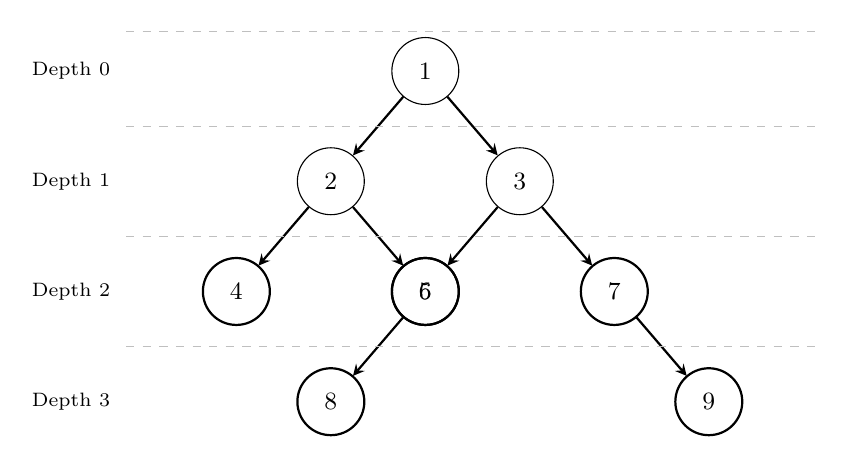
\begin{tikzpicture}[
  every node/.style={circle, draw, minimum size=0.85cm, font=\small, inner sep=1pt},
  level distance=1.4cm,
  sibling distance=2.4cm,
  edge from parent/.style={draw, ->, >=stealth, thick}
]
\node {1}
  child { node {2}
    child { node {4} }
    child { node {5}
      child { node {8} }
      child[missing] {}
    }
  }
  child { node {3}
    child { node {6} }
    child { node {7}
      child[missing] {}
      child { node {9} }
    }
  };

\node[draw=none, minimum size=0pt, font=\scriptsize] at (-4.5, 0) {Depth 0};
\node[draw=none, minimum size=0pt, font=\scriptsize] at (-4.5, -1.4) {Depth 1};
\node[draw=none, minimum size=0pt, font=\scriptsize] at (-4.5, -2.8) {Depth 2};
\node[draw=none, minimum size=0pt, font=\scriptsize] at (-4.5, -4.2) {Depth 3};

\draw[dashed, gray!50] (-3.8, 0.5) -- (5.0, 0.5);
\draw[dashed, gray!50] (-3.8, -0.7) -- (5.0, -0.7);
\draw[dashed, gray!50] (-3.8, -2.1) -- (5.0, -2.1);
\draw[dashed, gray!50] (-3.8, -3.5) -- (5.0, -3.5);

\end{tikzpicture}
\caption{Reference binary tree $T$ with 9 nodes used throughout this paper. Height $h = 3$. Nodes 4, 8, 6, and 9 are leaf nodes.}
\label{fig:reference_tree}
\end{figure}

\section{Recursive DFS Traversals}
\label{sec:recursive}

The recursive formulation of DFS leverages the programming language's call stack to manage the traversal state. Each recursive call pushes a new frame onto the stack containing the local variable (the current node pointer). When the call returns, the frame is popped and execution resumes at the caller.

\subsection{Pre-order Traversal (Root $\to$ Left $\to$ Right)}

\begin{definition}[Pre-order]
Given a binary tree rooted at node $r$, the pre-order traversal visits $r$, then recursively visits the left subtree $T_L$, then recursively visits the right subtree $T_R$.
\end{definition}

\begin{verbatim}
ArrayList<Integer> preorderTraversal(TreeNode root) {
    ArrayList<Integer> result = new ArrayList<>();
    preorderHelper(root, result);
    return result;
}

void preorderHelper(TreeNode node, ArrayList<Integer> result) {
    if (node == null) return;       // Base case
    result.add(node.val);           // Process root FIRST
    preorderHelper(node.left, result);   // Recurse left
    preorderHelper(node.right, result);  // Recurse right
}
\end{verbatim}

\textbf{Pre-order output for Figure~\ref{fig:reference_tree}:} $1, 2, 4, 5, 8, 3, 6, 7, 9$

\textbf{Key Insight:} In pre-order, the root is always the \emph{first} element in the output. This property is exploited in tree construction algorithms (Section~\ref{sec:applications}).

\subsection{In-order Traversal (Left $\to$ Root $\to$ Right)}

\begin{definition}[In-order]
Given a binary tree rooted at node $r$, the in-order traversal recursively visits the left subtree $T_L$, then visits $r$, then recursively visits the right subtree $T_R$.
\end{definition}

\begin{verbatim}
ArrayList<Integer> inorderTraversal(TreeNode A) {
    ArrayList<Integer> result = new ArrayList<>();
    inorderHelper(A, result);
    return result;
}

void inorderHelper(TreeNode node, ArrayList<Integer> result) {
    if (node == null) return;       // Base case
    inorderHelper(node.left, result);    // Recurse left FIRST
    result.add(node.val);                // Process root
    inorderHelper(node.right, result);   // Recurse right
}
\end{verbatim}

\textbf{In-order output for Figure~\ref{fig:reference_tree}:} $4, 2, 8, 5, 1, 6, 3, 7, 9$

\textbf{Key Insight:} For a Binary Search Tree (BST), in-order traversal produces elements in sorted (non-decreasing) order. This is because the BST invariant guarantees $\mathrm{left.val} < \mathrm{root.val} < \mathrm{right.val}$.

\subsection{Post-order Traversal (Left $\to$ Right $\to$ Root)}

\begin{definition}[Post-order]
Given a binary tree rooted at node $r$, the post-order traversal recursively visits the left subtree $T_L$, then recursively visits the right subtree $T_R$, then visits $r$.
\end{definition}

\begin{verbatim}
ArrayList<Integer> postorderTraversal(TreeNode root) {
    ArrayList<Integer> result = new ArrayList<>();
    postorderHelper(root, result);
    return result;
}

void postorderHelper(TreeNode node, ArrayList<Integer> result) {
    if (node == null) return;       // Base case
    postorderHelper(node.left, result);  // Recurse left
    postorderHelper(node.right, result); // Recurse right
    result.add(node.val);                // Process root LAST
}
\end{verbatim}

\textbf{Post-order output for Figure~\ref{fig:reference_tree}:} $4, 8, 5, 2, 6, 9, 7, 3, 1$

\textbf{Key Insight:} In post-order, the root is always the \emph{last} element in the output. Post-order is used for tree deletion (children must be freed before parent) and evaluating expression trees.

\subsection{Traversal Summary}

\begin{table}[htbp]
\centering
\caption{DFS Traversal Outputs for the Reference Tree (Figure~\ref{fig:reference_tree}).}
\label{tab:traversal_outputs}
\begin{tabular}{lll}
\toprule
Strategy & Order & Output Sequence \\
\midrule
Pre-order & Root-Left-Right & $1, 2, 4, 5, 8, 3, 6, 7, 9$ \\
In-order & Left-Root-Right & $4, 2, 8, 5, 1, 6, 3, 7, 9$ \\
Post-order & Left-Right-Root & $4, 8, 5, 2, 6, 9, 7, 3, 1$ \\
\bottomrule
\end{tabular}
\end{table}

\section{Call Stack Mechanics During DFS}
\label{sec:callstack}

Understanding the call stack is essential for analyzing the space complexity of recursive DFS and for developing iterative alternatives. We trace the \textbf{in-order traversal} on a small subtree to illustrate the stack frame dynamics.

\begin{figure}[htbp]
\centering
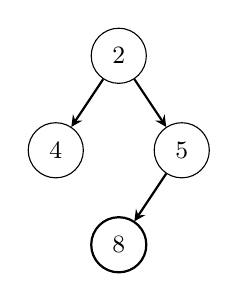
\begin{tikzpicture}[
  every node/.style={circle, draw, minimum size=0.7cm, font=\small, inner sep=1pt},
  level distance=1.2cm,
  sibling distance=1.6cm,
  edge from parent/.style={draw, ->, >=stealth, thick}
]
\node {2}
  child { node {4} }
  child { node {5}
    child { node {8} }
    child[missing] {}
  };
\end{tikzpicture}
\caption{Subtree rooted at node 2 used for call stack trace.}
\label{fig:subtree_trace}
\end{figure}

\begin{table}[htbp]
\centering
\caption{Call Stack Trace for In-order Traversal of Subtree Rooted at Node 2.}
\label{tab:callstack_trace}
\begin{tabular}{clll}
\toprule
Step & Action & Call Stack (top $\to$ bottom) & Output \\
\midrule
1 & Call inorder(2) & $[\text{inorder}(2)]$ & -- \\
2 & Call inorder(4) & $[\text{inorder}(4), \text{inorder}(2)]$ & -- \\
3 & Call inorder(null) & $[\text{null}, \text{inorder}(4), \text{inorder}(2)]$ & -- \\
4 & Return from null & $[\text{inorder}(4), \text{inorder}(2)]$ & -- \\
5 & Print 4 & $[\text{inorder}(4), \text{inorder}(2)]$ & 4 \\
6 & Call inorder(null) & $[\text{null}, \text{inorder}(4), \text{inorder}(2)]$ & 4 \\
7 & Return from null & $[\text{inorder}(4), \text{inorder}(2)]$ & 4 \\
8 & Return from 4 & $[\text{inorder}(2)]$ & 4 \\
9 & Print 2 & $[\text{inorder}(2)]$ & 4, 2 \\
10 & Call inorder(5) & $[\text{inorder}(5), \text{inorder}(2)]$ & 4, 2 \\
11 & Call inorder(8) & $[\text{inorder}(8), ..., \text{inorder}(2)]$ & 4, 2 \\
12 & inorder(null), return & stack unwinds & 4, 2 \\
13 & Print 8 & $[\text{inorder}(8), ..., \text{inorder}(2)]$ & 4, 2, 8 \\
14 & inorder(null), return & stack unwinds & 4, 2, 8 \\
15 & Return from 8 & $[\text{inorder}(5), \text{inorder}(2)]$ & 4, 2, 8 \\
16 & Print 5 & $[\text{inorder}(5), \text{inorder}(2)]$ & 4, 2, 8, 5 \\
17 & inorder(null), return & stack unwinds & 4, 2, 8, 5 \\
18 & Return from 5, 2 & $[\;]$ & 4, 2, 8, 5 \\
\bottomrule
\end{tabular}
\end{table}

\subsection{Space Complexity from the Call Stack}
\begin{theorem}
The auxiliary space complexity of recursive DFS on a binary tree is $O(H)$, where $H$ is the height of the tree.
\end{theorem}
\begin{proof}
At any point during execution, the call stack contains one frame per node on the path from the root to the current node being processed. The maximum number of simultaneous stack frames equals the length of the longest root-to-leaf path, which is the height $H$ of the tree. For a balanced tree, $H = O(\log N)$; for a completely skewed tree (linked-list shape), $H = N - 1 = O(N)$.
\end{proof}

\section{Iterative DFS Using Explicit Stacks}
\label{sec:iterative}

While the recursive implementations are elegant and concise, they suffer from potential stack overflow for deeply nested trees (e.g., skewed trees with $N > 10^5$ nodes). We can eliminate recursion by using an explicit \texttt{Stack} data structure. This converts the implicit call stack into a programmer-controlled stack, maintaining the same $O(H)$ space complexity but avoiding system stack limitations.

\subsection{Iterative Pre-order Traversal}

Pre-order is the simplest to convert iteratively. We push the root, then repeatedly pop a node, process it, and push its right child first (so left is processed first due to LIFO order).

\begin{verbatim}
import java.util.Stack;

ArrayList<Integer> preorderIterative(TreeNode root) {
    ArrayList<Integer> result = new ArrayList<>();
    if (root == null) return result;

    Stack<TreeNode> stack = new Stack<>();
    stack.push(root);

    while (!stack.isEmpty()) {
        TreeNode curr = stack.pop();
        result.add(curr.val);        // Process current

        // Push right first so left is processed first (LIFO)
        if (curr.right != null) stack.push(curr.right);
        if (curr.left != null) stack.push(curr.left);
    }
    return result;
}
\end{verbatim}

\subsection{Iterative In-order Traversal}

In-order is more nuanced. We must go as far left as possible before processing any node. We use a pointer \texttt{curr} and push nodes until we hit \texttt{null}, then pop and process, and move to the right subtree.

\begin{verbatim}
ArrayList<Integer> inorderIterative(TreeNode root) {
    ArrayList<Integer> result = new ArrayList<>();
    Stack<TreeNode> stack = new Stack<>();
    TreeNode curr = root;

    while (curr != null || !stack.isEmpty()) {
        // Go as far left as possible
        while (curr != null) {
            stack.push(curr);
            curr = curr.left;
        }
        // Process the leftmost unprocessed node
        curr = stack.pop();
        result.add(curr.val);
        // Move to right subtree
        curr = curr.right;
    }
    return result;
}
\end{verbatim}

\begin{table}[htbp]
\centering
\caption{Step-by-step Iterative In-order Trace for the Left Subtree (Nodes 2, 4, 5, 8).}
\label{tab:iter_inorder_trace}
\begin{tabular}{cllll}
\toprule
Step & curr & Action & Stack (top $\to$) & Output \\
\midrule
1 & 2 & Push 2, go left & $[2]$ & -- \\
2 & 4 & Push 4, go left & $[4, 2]$ & -- \\
3 & null & Pop 4, print, go right & $[2]$ & 4 \\
4 & null & Pop 2, print, go right & $[\;]$ & 4, 2 \\
5 & 5 & Push 5, go left & $[5]$ & 4, 2 \\
6 & 8 & Push 8, go left & $[8, 5]$ & 4, 2 \\
7 & null & Pop 8, print, go right & $[5]$ & 4, 2, 8 \\
8 & null & Pop 5, print, go right & $[\;]$ & 4, 2, 8, 5 \\
9 & null & Stack empty, done & $[\;]$ & 4, 2, 8, 5 \\
\bottomrule
\end{tabular}
\end{table}

\subsection{Iterative Post-order Traversal Using Two Stacks}

Post-order is the most complex iteratively. A clean approach uses two stacks. We perform a modified pre-order (Root-Right-Left) into \texttt{st2}, then pop \texttt{st2} to get Left-Right-Root order.

\begin{verbatim}
ArrayList<Integer> postorderIterative(TreeNode root) {
    ArrayList<Integer> result = new ArrayList<>();
    if (root == null) return result;

    Stack<TreeNode> st1 = new Stack<>();
    Stack<TreeNode> st2 = new Stack<>();
    st1.push(root);

    while (!st1.isEmpty()) {
        TreeNode curr = st1.pop();
        st2.push(curr);
        // Push left first, then right (reverse of post-order)
        if (curr.left != null) st1.push(curr.left);
        if (curr.right != null) st1.push(curr.right);
    }

    while (!st2.isEmpty()) {
        result.add(st2.pop().val);
    }
    return result;
}
\end{verbatim}

\textbf{Why this works:} \texttt{st1} produces nodes in Root-Right-Left order. Pushing these into \texttt{st2} reverses the order to Left-Right-Root, which is exactly post-order.

\subsection{Complexity Comparison of Iterative Variants}

\begin{table}[htbp]
\centering
\caption{Complexity of Iterative DFS Variants.}
\label{tab:iterative_complexity}
\begin{tabular}{lccc}
\toprule
Algorithm & Time & Aux. Space & Stacks Used \\
\midrule
Iterative Pre-order & $O(N)$ & $O(H)$ & 1 \\
Iterative In-order & $O(N)$ & $O(H)$ & 1 \\
Iterative Post-order (2-stack) & $O(N)$ & $O(N)$ & 2 \\
\bottomrule
\end{tabular}
\end{table}

\section{Morris Traversal: $O(1)$ Space In-order DFS}
\label{sec:morris}

Morris Traversal achieves in-order traversal using $O(1)$ auxiliary space by temporarily modifying the tree structure. It creates \emph{threaded links} from in-order predecessors back to their successors, eliminating the need for a stack.

\subsection{Algorithm Description}
For each node, we find its \emph{in-order predecessor} (the rightmost node in its left subtree):
\begin{enumerate}
    \item If the left subtree is \texttt{null}, process the current node and move right.
    \item If the left subtree exists, find the in-order predecessor $p$:
    \begin{enumerate}
        \item If $p.\texttt{right} == \texttt{null}$: Set $p.\texttt{right} = \texttt{curr}$ (create thread), move left.
        \item If $p.\texttt{right} == \texttt{curr}$: Remove the thread ($p.\texttt{right} = \texttt{null}$), process \texttt{curr}, move right.
    \end{enumerate}
\end{enumerate}

\subsection{Java Implementation}
\begin{verbatim}
ArrayList<Integer> morrisInorder(TreeNode root) {
    ArrayList<Integer> result = new ArrayList<>();
    TreeNode curr = root;

    while (curr != null) {
        if (curr.left == null) {
            // No left subtree: process and go right
            result.add(curr.val);
            curr = curr.right;
        } else {
            // Find in-order predecessor
            TreeNode pred = curr.left;
            while (pred.right != null && pred.right != curr) {
                pred = pred.right;
            }

            if (pred.right == null) {
                // Create thread: predecessor -> current
                pred.right = curr;
                curr = curr.left;
            } else {
                // Thread exists: remove it, process current
                pred.right = null;
                result.add(curr.val);
                curr = curr.right;
            }
        }
    }
    return result;
}
\end{verbatim}

\begin{figure}[htbp]
\centering
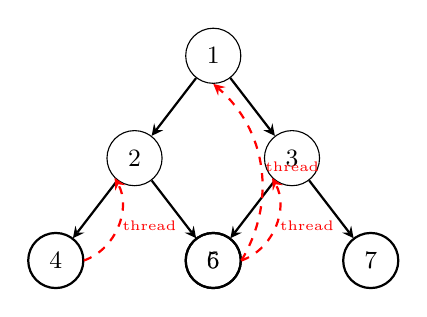
\begin{tikzpicture}[
  every node/.style={circle, draw, minimum size=0.7cm, font=\small, inner sep=1pt},
  level distance=1.3cm,
  sibling distance=2.0cm,
  edge from parent/.style={draw, ->, >=stealth, thick}
]
\node (n1) {1}
  child { node (n2) {2}
    child { node (n4) {4} }
    child { node (n5) {5} }
  }
  child { node (n3) {3}
    child { node (n6) {6} }
    child { node (n7) {7} }
  };

% Draw Morris threads as dashed red arrows
\draw[->, >=stealth, dashed, red, thick, bend right=50] (n4.east) to node[draw=none, minimum size=0pt, font=\tiny, right, red] {thread} (n2.south west);
\draw[->, >=stealth, dashed, red, thick, bend right=40] (n5.east) to node[draw=none, minimum size=0pt, font=\tiny, right, red] {thread} (n1.south);
\draw[->, >=stealth, dashed, red, thick, bend right=50] (n6.east) to node[draw=none, minimum size=0pt, font=\tiny, right, red] {thread} (n3.south west);

\end{tikzpicture}
\caption{Morris Traversal threads (dashed red arrows). Node 4 (in-order predecessor of 2) threads to 2. Node 5 (in-order predecessor of 1) threads to 1. Node 6 (in-order predecessor of 3) threads to 3. These threads are temporary and removed after processing.}
\label{fig:morris_threads}
\end{figure}

\subsection{Complexity Analysis}
\begin{theorem}
Morris Traversal runs in $O(N)$ time and $O(1)$ auxiliary space.
\end{theorem}
\begin{proof}
\textbf{Time:} Each edge in the tree is traversed at most 3 times: once during the initial traversal, once to create a thread, and once to remove the thread. Since a binary tree with $N$ nodes has $N - 1$ edges, the total traversals are bounded by $3(N-1) = O(N)$.

\textbf{Space:} No additional data structures (stacks, queues, or hash maps) are allocated. The threads temporarily reuse existing \texttt{null} right pointers. The tree structure is fully restored after traversal. Hence, auxiliary space is $O(1)$.
\end{proof}

\section{DFS Applications on Binary Trees}
\label{sec:applications}

DFS serves as the backbone for solving a wide range of binary tree problems. We present four classic applications.

\subsection{Application 1: Computing Tree Height}

The height of a binary tree is the number of edges on the longest root-to-leaf path. We compute it via post-order DFS: the height of a node is $1 + \max(\text{height}(\text{left}), \text{height}(\text{right}))$.

\begin{verbatim}
int height(TreeNode root) {
    if (root == null) return -1;  // Height of empty tree is -1
    int leftH = height(root.left);
    int rightH = height(root.right);
    return 1 + Math.max(leftH, rightH);
}
\end{verbatim}

\textbf{For the reference tree:} $\text{height}(1) = 1 + \max(2, 2) = 3$.

\subsection{Application 2: Diameter of a Binary Tree}

\begin{definition}[Diameter]
The \emph{diameter} of a binary tree is the length of the longest path between any two nodes. This path may or may not pass through the root.
\end{definition}

The diameter through any node $v$ is $\text{height}(v.\text{left}) + \text{height}(v.\text{right}) + 2$. The global diameter is the maximum across all nodes.

\begin{verbatim}
int diameter = 0;

int computeDiameter(TreeNode root) {
    if (root == null) return -1;
    int leftH = computeDiameter(root.left);
    int rightH = computeDiameter(root.right);
    // Update global diameter
    diameter = Math.max(diameter, leftH + rightH + 2);
    return 1 + Math.max(leftH, rightH);
}
\end{verbatim}

This runs in $O(N)$ time since we compute height and diameter in a single DFS pass.

\subsection{Application 3: Path Sum Detection}

Given a target sum $S$, determine if there exists a root-to-leaf path whose node values sum to $S$.

\begin{verbatim}
boolean hasPathSum(TreeNode root, int targetSum) {
    if (root == null) return false;
    // Leaf node check
    if (root.left == null && root.right == null) {
        return root.val == targetSum;
    }
    int remaining = targetSum - root.val;
    return hasPathSum(root.left, remaining) ||
           hasPathSum(root.right, remaining);
}
\end{verbatim}

The DFS explores all root-to-leaf paths, subtracting each node's value from the remaining sum. When a leaf is reached, we check if the remaining sum equals the leaf's value.

\subsection{Application 4: Constructing a Tree from In-order and Pre-order}

\begin{theorem}
A binary tree can be uniquely reconstructed from its in-order and pre-order traversal sequences (assuming all node values are distinct).
\end{theorem}
\begin{proof}[Proof sketch]
The first element of the pre-order sequence is the root. We find this root's position $i$ in the in-order sequence. Elements to the left of $i$ in in-order form the left subtree; elements to the right form the right subtree. We recurse on both halves, advancing through the pre-order sequence to identify sub-roots.
\end{proof}

\begin{verbatim}
import java.util.HashMap;

TreeNode buildTree(int[] preorder, int[] inorder) {
    HashMap<Integer, Integer> inMap = new HashMap<>();
    for (int i = 0; i < inorder.length; i++) {
        inMap.put(inorder[i], i);
    }
    return build(preorder, 0, preorder.length - 1,
                 inorder, 0, inorder.length - 1, inMap);
}

int preIdx = 0;

TreeNode build(int[] pre, int preStart, int preEnd,
               int[] in, int inStart, int inEnd,
               HashMap<Integer, Integer> inMap) {
    if (preStart > preEnd || inStart > inEnd) return null;

    TreeNode root = new TreeNode(pre[preStart]);
    int inRoot = inMap.get(root.val);
    int leftSize = inRoot - inStart;

    root.left = build(pre, preStart + 1, preStart + leftSize,
                      in, inStart, inRoot - 1, inMap);
    root.right = build(pre, preStart + leftSize + 1, preEnd,
                       in, inRoot + 1, inEnd, inMap);
    return root;
}
\end{verbatim}

The HashMap provides $O(1)$ root lookups in the in-order array, giving an overall $O(N)$ time complexity.

\section{Comprehensive Complexity Summary}

\begin{table}[htbp]
\centering
\caption{Complete Complexity Analysis of All DFS Algorithms.}
\label{tab:full_complexity}
\begin{tabular}{lccl}
\toprule
Algorithm & Time & Aux. Space & Notes \\
\midrule
Recursive Pre-order & $O(N)$ & $O(H)$ & Call stack \\
Recursive In-order & $O(N)$ & $O(H)$ & Call stack \\
Recursive Post-order & $O(N)$ & $O(H)$ & Call stack \\
Iterative Pre-order & $O(N)$ & $O(H)$ & 1 explicit stack \\
Iterative In-order & $O(N)$ & $O(H)$ & 1 explicit stack \\
Iterative Post-order & $O(N)$ & $O(N)$ & 2 explicit stacks \\
Morris In-order & $O(N)$ & $O(1)$ & Temporary threads \\
Height Computation & $O(N)$ & $O(H)$ & Post-order DFS \\
Diameter Computation & $O(N)$ & $O(H)$ & Single DFS pass \\
Path Sum Detection & $O(N)$ & $O(H)$ & Pre-order DFS \\
Tree Construction & $O(N)$ & $O(N)$ & HashMap + recursion \\
\bottomrule
\end{tabular}
\end{table}

\noindent where $N$ is the number of nodes and $H$ is the height of the tree. For balanced trees, $H = O(\log N)$. For skewed trees, $H = O(N)$.

\section{Conclusion}

This paper has presented a comprehensive formal treatment of Depth-First Search on binary trees. We established the three canonical DFS orderings --- Pre-order, In-order, and Post-order --- providing both recursive and iterative Java implementations. We dissected the call stack mechanics frame-by-frame, proving the $O(H)$ space bound. We developed iterative equivalents using explicit stacks, demonstrating their correctness through detailed execution traces. We introduced Morris Traversal as an elegant $O(1)$ auxiliary space alternative for in-order traversal that temporarily threads the tree structure. Finally, we applied DFS to four classic binary tree problems: height computation, diameter calculation, path sum detection, and tree reconstruction from traversal pairs. The recursive nature of binary trees makes DFS the natural and often optimal traversal paradigm, with each variant offering distinct advantages depending on the problem's structural requirements.

\end{document}
